\chapter{Matriisit}

\index{matriisi}

Matriisi on kaksiulotteista taulukkoa
vastaava matemaattinen käsite,
jolle on määritelty laskutoimituksia.
Esimerkiksi
\[
A = 
 \begin{bmatrix}
  6 & 13 & 7 & 4 \\
  7 & 0 & 8 & 2 \\
  9 & 5 & 4 & 18 \\
 \end{bmatrix}
\]
on matriisi, jossa on 3 riviä ja 4 saraketta
eli se on kokoa $3 \times 4$.
Matriisin alkioihin on mahdollista
viitata merkinnällä $[i,j]$,
jossa $i$ on rivi ja $j$ on sarake.
Esimerkiksi yllä olevassa matriisissa
$A[2,3]=8$ ja $A[3,1]=9$.

\index{vektori}

Matriisin erikoistapaus on \textit{vektori},
joka on kokoa $n \times 1$ oleva yksiulotteinen matriisi.
Esimerkiksi
\[
V =
\begin{bmatrix}
4 \\
7 \\
5 \\
\end{bmatrix}
\]
on vektori, jossa on 3 alkiota.

\index{transpoosi}

Matriisin $A$ \textit{transpoosi} $A^T$ syntyy,
kun matriisin rivit ja sarakkeet vaihdetaan
keskenään eli $A^T[i,j]=A[j,i]$:
\[
A^T = 
 \begin{bmatrix}
  6 & 7 & 9 \\
  13 & 0 & 5 \\
  7 & 8 & 4 \\
  4 & 2 & 18 \\
 \end{bmatrix}
\]

\index{neliömatriisi}

Matriisi on \textit{neliömatriisi}, jos sen
korkeus ja leveys ovat samat.
Esimerkiksi seuraava matriisi on neliömatriisi:

\[
A = 
 \begin{bmatrix}
  3 & 12 & 4  \\
  5 & 9 & 15  \\
  0 & 2 & 4 \\
 \end{bmatrix}
\]

\section{Laskutoimitukset}

Matriisien $A$ ja $B$ summa $A+B$ on määritelty,
jos matriisit ovat yhtä suuret.
Tuloksena oleva matriisi on
samaa kokoa kuin
matriisit $A$ ja $B$ ja sen jokainen
alkio on vastaavissa kohdissa
olevien alkioiden summa.

Esimerkiksi
\[
 \begin{bmatrix}
  6 & 1 & 4 \\
  3 & 9 & 2 \\
 \end{bmatrix}
+
 \begin{bmatrix}
  4 & 9 & 3 \\
  8 & 1 & 3 \\
 \end{bmatrix}
=
 \begin{bmatrix}
  6+4 & 1+9 & 4+3 \\
  3+8 & 9+1 & 2+3 \\
 \end{bmatrix}
=
 \begin{bmatrix}
  10 & 10 & 7 \\
  11 & 10 & 5 \\
 \end{bmatrix}.
\]

Matriisin $A$ kertominen luvulla $x$ tarkoittaa,
että jokainen matriisin alkio kerrotaan luvulla $x$.

Esimerkiksi
\[
 2 \cdot \begin{bmatrix}
  6 & 1 & 4 \\
  3 & 9 & 2 \\
 \end{bmatrix}
=
 \begin{bmatrix}
  2 \cdot 6 & 2\cdot1 & 2\cdot4 \\
  2\cdot3 & 2\cdot9 & 2\cdot2 \\
 \end{bmatrix}
=
 \begin{bmatrix}
  12 & 2 & 8 \\
  6 & 18 & 4 \\
 \end{bmatrix}.
\]

\subsubsection{Matriisitulo}

\index{matriisitulo}

Matriisien $A$ ja $B$ tulo $AB$ on määritelty,
jos matriisi $A$ on kokoa $a \times n$
ja matriisi $B$ on kokoa $n \times b$,
eli matriisin $A$ leveys on sama kuin matriisin
$B$ korkeus.
Tuloksena oleva matriisi
on kokoa $a \times b$
ja sen alkiot lasketaan kaavalla
\[
AB[i,j] = \sum_{k=1}^n A[i,k] \cdot B[k,j].
\]

Kaavan tulkintana on, että kukin $AB$:n alkio
saadaan summana, joka muodostuu $A$:n ja
$B$:n alkioparien tuloista seuraavan
kuvan mukaisesti:

\begin{center}
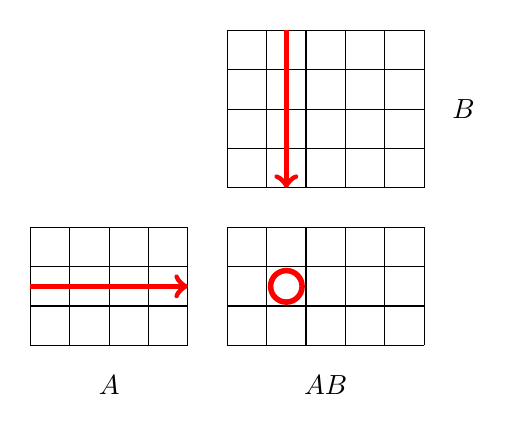
\begin{tikzpicture}[scale=0.5]
\draw (0,0) grid (4,3);
\draw (5,0) grid (10,3);
\draw (5,4) grid (10,8);

\node at (2,-1) {$A$};
\node at (7.5,-1) {$AB$};
\node at (11,6) {$B$};

\draw[thick,->,red,line width=2pt] (0,1.5) -- (4,1.5);
\draw[thick,->,red,line width=2pt] (6.5,8) -- (6.5,4);
\draw[thick,red,line width=2pt] (6.5,1.5) circle (0.4);
\end{tikzpicture}
\end{center}

Esimerkiksi

\[
 \begin{bmatrix}
  1 & 4 \\
  3 & 9 \\
  8 & 6 \\
 \end{bmatrix}
\cdot
 \begin{bmatrix}
  1 & 6 \\
  2 & 9 \\
 \end{bmatrix}
=
 \begin{bmatrix}
  1 \cdot 1 + 4 \cdot 2 & 1 \cdot 6 + 4 \cdot 9 \\
  3 \cdot 1 + 9 \cdot 2 & 3 \cdot 6 + 9 \cdot 9 \\
  8 \cdot 1 + 6 \cdot 2 & 8 \cdot 6 + 6 \cdot 9 \\
 \end{bmatrix}
=
 \begin{bmatrix}
  9 & 42 \\
  21 & 99 \\
  20 & 102 \\
 \end{bmatrix}.
\]

Matriisitulo ei ole vaihdannainen,
eli ei ole voimassa $A \cdot B = B \cdot A$.
Kuitenkin matriisitulo
on liitännäinen, eli on voimassa $A \cdot (B \cdot C)=(A \cdot B) \cdot C$.

\index{ykkösmatriisi}

\textit{Ykkösmatriisi} on neliömatriisi,
jonka lävistäjän jokainen alkio on 1
ja jokainen muu alkio on 0.
Esimerkiksi $3 \times 3$ -yksikkömatriisi on
seuraavanlainen:
\[
 I = \begin{bmatrix}
  1 & 0 & 0 \\
  0 & 1 & 0 \\
  0 & 0 & 1 \\
 \end{bmatrix}
\]

\begin{samepage}
Ykkösmatriisilla kertominen säilyttää matriisin
ennallaan. Esimerkiksi
\[
 \begin{bmatrix}
  1 & 0 & 0 \\
  0 & 1 & 0 \\
  0 & 0 & 1 \\
 \end{bmatrix}
\cdot
 \begin{bmatrix}
  1 & 4 \\
  3 & 9 \\
  8 & 6 \\
 \end{bmatrix}
=
 \begin{bmatrix}
  1 & 4 \\
  3 & 9 \\
  8 & 6 \\
 \end{bmatrix} \hspace{10px} \textrm{ja} \hspace{10px}
 \begin{bmatrix}
  1 & 4 \\
  3 & 9 \\
  8 & 6 \\
 \end{bmatrix}
\cdot
 \begin{bmatrix}
  1 & 0 \\
  0 & 1 \\
 \end{bmatrix}
=
 \begin{bmatrix}
  1 & 4 \\
  3 & 9 \\
  8 & 6 \\
 \end{bmatrix}.
\]
\end{samepage}

Matriisitulon laskeminen vie aikaa $O(n^3)$
käyttäen suoraviivaista algoritmia,
kun $A$ ja $B$ ovat kokoa $n \times n$.
Myös nopeampia algoritmeja on olemassa,
mutta ne eivät ole tarpeen kisakoodauksessa.

\subsubsection{Matriisipotenssi}

\index{matriisipotenssi}

Matriisin $A$ potenssi $A^k$ on
määritelty, jos $A$ on neliömatriisi.
Määritelmä nojautuu kertolaskuun:
\[ A^k = \underbrace{A \cdot A \cdot A \cdots A}_{\textrm{$k$ kertaa}} \]
Esimerkiksi

\[
 \begin{bmatrix}
  2 & 5 \\
  1 & 4 \\
 \end{bmatrix}^3 =
 \begin{bmatrix}
  2 & 5 \\
  1 & 4 \\
 \end{bmatrix} \cdot
 \begin{bmatrix}
  2 & 5 \\
  1 & 4 \\
 \end{bmatrix} \cdot
 \begin{bmatrix}
  2 & 5 \\
  1 & 4 \\
 \end{bmatrix} =
 \begin{bmatrix}
  48 & 165 \\
  33 & 114 \\
 \end{bmatrix}.
\]
Lisäksi $A^0$ tuottaa ykkösmatriisin. Esimerkiksi
\[
 \begin{bmatrix}
  2 & 5 \\
  1 & 4 \\
 \end{bmatrix}^0 =
 \begin{bmatrix}
  1 & 0 \\
  0 & 1 \\
 \end{bmatrix}.
\]

Matriisin $A^k$ voi laskea tehokkaasti ajassa
$O(n^3 \log k)$ soveltamalla luvun 21.2
tehokasta potenssilaskua. Esimerkiksi
\[
 \begin{bmatrix}
  2 & 5 \\
  1 & 4 \\
 \end{bmatrix}^8 =
 \begin{bmatrix}
  2 & 5 \\
  1 & 4 \\
 \end{bmatrix}^4 \cdot
 \begin{bmatrix}
  2 & 5 \\
  1 & 4 \\
 \end{bmatrix}^4.
\]


\subsubsection{Determinantti}

\index{determinantti}

Matriisin $A$ \textit{determinantti} $\det(A)$
on määritelty, jos $A$ on neliömatriisi.
Jos $A$ on kokoa $1 \times 1$,
niin $\det(A)=A[1,1]$.
Muuten determinaatti lasketaan rekursiivisesti
kaavalla

\[\det(A)=\sum_{j=1}^n A[1,j] C[1,j],\]

\index{kofaktori}

missä $C[i,j]$ on matriisin $A$ \textit{kofaktori}
kohdassa $[i,j]$.
Kofaktori lasketaan kaavalla

\[C[i,j] = (-1)^{i+j} A'[i,j],\]

missä $A'$ on matriisi $A$, josta on poistettu
rivi $i$ ja sarake $j$.
Kofaktorissa olevan kertoimen $(-1)^{i+j}$ ansiosta
joka toinen determinantti
lisätään summaan positiivisena
ja joka toinen negatiivisena.

\begin{samepage}
Esimerkiksi
\[
\det(
 \begin{bmatrix}
  3 & 4 \\
  1 & 6 \\
 \end{bmatrix}
) = 3 \cdot 6 - 4 \cdot 1 = 14 
\]
\end{samepage}

ja

\[
\det(
 \begin{bmatrix}
  2 & 4 & 3 \\
  5 & 1 & 6 \\
  7 & 2 & 4 \\
 \end{bmatrix}
) = 
2 \cdot
\det(
 \begin{bmatrix}
  1 & 6 \\
  2 & 4 \\
 \end{bmatrix}
)
-4 \cdot
\det(
 \begin{bmatrix}
  5 & 6 \\
  7 & 4 \\
 \end{bmatrix}
)
+3 \cdot
\det(
 \begin{bmatrix}
  5 & 1 \\
  7 & 2 \\
 \end{bmatrix}
) = 81.
\]

\index{käänteismatriisi}

Determinantti kertoo, onko matriisille
$A$ olemassa \textit{käänteismatriisia}
$A^{-1}$, jolle pätee $A \cdot A^{-1} = I$,
missä $I$ on ykkösmatriisi.
Osoittautuu, että $A^{-1}$ on olemassa
tarkalleen silloin, kun $\det(A) \neq 0$,
ja sen voi laskea kaavalla

\[A^{-1}[i,j] = \frac{C[j,i]}{det(A)}.\]

Esimerkiksi

\[
\underbrace{
 \begin{bmatrix}
  2 & 4 & 3\\
  5 & 1 & 6\\
  7 & 2 & 4\\
 \end{bmatrix}
}_{A}
\cdot
\underbrace{
 \frac{1}{81}
 \begin{bmatrix}
   -8 & -10 & 21 \\
   22 & -13 & 3 \\
   3 & 24 & -18 \\
 \end{bmatrix}
}_{A^{-1}}
=
\underbrace{
 \begin{bmatrix}
  1 & 0 & 0 \\
  0 & 1 & 0 \\
  0 & 0 & 1 \\
 \end{bmatrix}
}_{I}.
\]

\section{Lineaariset rekursioyhtälöt}

\index{rekursioyhtälö}

Lineaarinen rekursioyhtälö 
voidaan esittää funktiona $f(n)$,
jolle on annettu alkuarvot
$f(0),f(1),\ldots,f(k-1)$
ja jonka suuremmat arvot
parametrista $k$ lähtien lasketaan
rekursiivisesti kaavalla
\[f(n) = c_1 f(n-1) + c_2 f(n-2) + \ldots + c_k f (n-k),\]
missä $c_1,c_2,\ldots,c_k$ ovat vakiokertoimia.

Funktion arvon $f(n)$ voi laskea dynaamisella
ohjelmoinnilla ajassa $O(kn)$
laskemalla kaikki arvot $f(0),f(1),\ldots,f(n)$ järjestyksessä.
Tätä ratkaisua voi kuitenkin tehostaa merkittävästi
matriisien avulla.
Seuraavaksi näemme, miten arvon $f(n)$
voi laskea ajassa $O(k^3 \log n)$.

\subsubsection{Fibonaccin luvut}

\index{Fibonaccin luku}

Yksinkertainen esimerkki lineaarisesta rekursioyhtälöstä
on Fibonaccin luvut määrittelevä funktio:
\[
\begin{array}{lcl}
f(0) & = & 0 \\
f(1) & = & 1 \\
f(n) & = & f(n-1)+f(n-2) \\
\end{array}
\]
Tässä tapauksessa $k=2$ ja $c_1=c_2=1$.

\begin{samepage}
Ideana on esittää rekursiivinen kaava $k \times k$
-kokoisena neliömatriisina $X$, jolle pätee
\[ X \cdot
 \begin{bmatrix}
  f(i) \\
  f(i+1) \\
 \end{bmatrix}
=
 \begin{bmatrix}
  f(i+1) \\
  f(i+2) \\
 \end{bmatrix}
 \]
\end{samepage}
eli $X$:lle annetaan
''syötteenä'' $k$ peräkkäistä funktion $f$ arvoa
kohdasta $i$ alkaen ja $X$ muodostaa niistä
$k$ peräkkäistä arvoa kohdasta $i+1$ alkaen.
Fibonaccin lukujen tapauksessa tällainen matriisi on

\[ X = 
 \begin{bmatrix}
  0 & 1 \\
  1 & 1 \\
 \end{bmatrix}.
\]

Esimerkiksi

\[
 \begin{bmatrix}
  0 & 1 \\
  1 & 1 \\
 \end{bmatrix}
\cdot
 \begin{bmatrix}
  f(5) \\
  f(6) \\
 \end{bmatrix}
=
 \begin{bmatrix}
  0 & 1 \\
  1 & 1 \\
 \end{bmatrix}
\cdot
 \begin{bmatrix}
  5 \\
  8 \\
 \end{bmatrix}
=
 \begin{bmatrix}
  8 \\
  13 \\
 \end{bmatrix}
=
 \begin{bmatrix}
  f(6) \\
  f(7) \\
 \end{bmatrix}.
\]

Tämän ansiosta arvon $f(n)$ sisältävän matriisin saa laskettua
kaavalla

\[
 \begin{bmatrix}
  f(n) \\
  f(n+1) \\
 \end{bmatrix}
=
X^n \cdot
 \begin{bmatrix}
  f(0) \\
  f(1) \\
 \end{bmatrix}
=
 \begin{bmatrix}
  0 & 1 \\
  1 & 1 \\
 \end{bmatrix}^n
\cdot
 \begin{bmatrix}
  0 \\
  1 \\
 \end{bmatrix}.
\]

Potenssilasku $X^n$ onnistuu ajassa
$O(k^3 \log n)$,
joten myös funktion arvon $f(n)$
saa laskettua ajassa $O(k^3 \log n)$.

\subsubsection{Yleinen tapaus}

Tarkastellaan sitten yleistä tapausta,
missä $f(n)$ on mikä tahansa lineaarinen
rekursioyhtälö. Nyt tavoitteena on etsiä
matriisi $X$, jolle pätee

\[ X \cdot
 \begin{bmatrix}
  f(i) \\
  f(i+1) \\
  \vdots \\
  f(i+k-1) \\
 \end{bmatrix}
=
 \begin{bmatrix}
  f(i+1) \\
  f(i+2) \\
  \vdots \\
  f(i+k) \\
 \end{bmatrix}.
\]

Tällainen matriisi on

\[
X =
 \begin{bmatrix}
  0 & 1 & 0 & 0 & \cdots & 0 \\
  0 & 0 & 1 & 0 & \cdots & 0 \\
  0 & 0 & 0 & 1 & \cdots & 0 \\
  \vdots & \vdots & \vdots & \vdots & \ddots & \vdots \\
  0 & 0 & 0 & 0 & \cdots & 1 \\
  c_k & c_{k-1} & c_{k-2} & c_{k-3} & \cdots & c_1 \\
 \end{bmatrix}.
\]
Matriisin $k-1$ ensimmäisen rivin jokainen alkio on 0,
paitsi yksi alkio on 1.
Nämä rivit kopioivat
arvon $f(i+1)$ arvon $f(i)$ tilalle,
arvon $f(i+2)$ arvon $f(i+1)$ tilalle jne.
Viimeinen rivi sisältää rekursiokaavan kertoimet,
joiden avulla muodostuu uusi arvo $f(i+k)$.

\begin{samepage}
Nyt arvon $f(n)$ pystyy laskemaan ajassa $O(k^3 \log n)$
kaavalla
\[
 \begin{bmatrix}
  f(n) \\
  f(n+1) \\
  \vdots \\
  f(n+k-1) \\
 \end{bmatrix}
=
X^n \cdot
 \begin{bmatrix}
  f(0) \\
  f(1) \\
  \vdots \\
  f(k-1) \\
 \end{bmatrix}.
\]
\end{samepage}

\section{Verkkojen käsittely}

Matriisipotenssilla
on mielenkiintoinen vaikutus
verkon vierusmatriisin sisältöön.
Kun $V$ on painottoman verkon vierusmatriisi,
niin $V^n$ kertoo,
montako $n$ kaaren pituista polkua
eri solmuista on toisiinsa.

Esimerkiksi verkon
\begin{center}
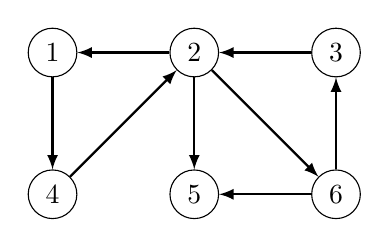
\begin{tikzpicture}[scale=0.9]
\node[draw, circle] (1) at (1,3) {$1$};
\node[draw, circle] (2) at (1,1) {$4$};
\node[draw, circle] (3) at (3,3) {$2$};
\node[draw, circle] (4) at (5,3) {$3$};
\node[draw, circle] (5) at (3,1) {$5$};
\node[draw, circle] (6) at (5,1) {$6$};

\path[draw,thick,->,>=latex] (1) -- (2);
\path[draw,thick,->,>=latex] (2) -- (3);
\path[draw,thick,->,>=latex] (3) -- (1);
\path[draw,thick,->,>=latex] (4) -- (3);
\path[draw,thick,->,>=latex] (3) -- (5);
\path[draw,thick,->,>=latex] (3) -- (6);
\path[draw,thick,->,>=latex] (6) -- (4);
\path[draw,thick,->,>=latex] (6) -- (5);
\end{tikzpicture}
\end{center}

vierusmatriisi on

\[
V= \begin{bmatrix}
  0 & 0 & 0 & 1 & 0 & 0 \\
  1 & 0 & 0 & 0 & 1 & 1 \\
  0 & 1 & 0 & 0 & 0 & 0 \\
  0 & 1 & 0 & 0 & 0 & 0 \\
  0 & 0 & 0 & 0 & 0 & 0 \\
  0 & 0 & 1 & 0 & 1 & 0 \\
 \end{bmatrix}.
\]

Nyt esimerkiksi matriisi
\[
V^4= \begin{bmatrix}
  0 & 0 & 1 & 1 & 1 & 0 \\
  2 & 0 & 0 & 0 & 2 & 2 \\
  0 & 2 & 0 & 0 & 0 & 0 \\
  0 & 2 & 0 & 0 & 0 & 0 \\
  0 & 0 & 0 & 0 & 0 & 0 \\
  0 & 0 & 1 & 1 & 1 & 0 \\
 \end{bmatrix}
\]

kertoo, montako 4 kaaren pituista polkua
solmuista on toisiinsa.
Esimerkiksi $V^4[2,5]=2$,
koska solmusta 2 solmuun 5 on olemassa
4 kaaren pituiset polut
$2 \rightarrow 1 \rightarrow 4 \rightarrow 2 \rightarrow 5$
ja 
$2 \rightarrow 6 \rightarrow 3 \rightarrow 2 \rightarrow 5$.

\subsubsection{Lyhimmät polut}

Samantapaisella idealla voi laskea painotetussa verkossa
kullekin solmuparille,
mikä on lyhin $n$ kaaren pituinen polku solmujen välillä.
Tämä vaatii matriisitulon määritelmän muuttamista
niin, että siinä ei lasketa polkujen yhteismäärää
vaan minimoidaan polun pituutta.

\begin{samepage}
Tarkastellaan esimerkkinä seuraavaa verkkoa:
\begin{center}
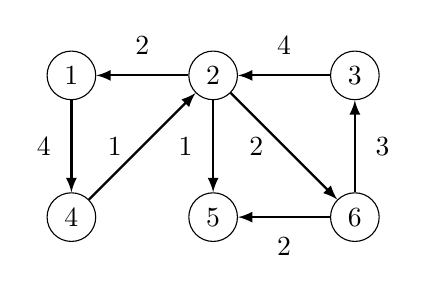
\begin{tikzpicture}[scale=0.9]
\node[draw, circle] (1) at (1,3) {$1$};
\node[draw, circle] (2) at (1,1) {$4$};
\node[draw, circle] (3) at (3,3) {$2$};
\node[draw, circle] (4) at (5,3) {$3$};
\node[draw, circle] (5) at (3,1) {$5$};
\node[draw, circle] (6) at (5,1) {$6$};

\path[draw,thick,->,>=latex] (1) -- node[font=\small,label=left:4] {} (2);
\path[draw,thick,->,>=latex] (2) -- node[font=\small,label=left:1] {} (3);
\path[draw,thick,->,>=latex] (3) -- node[font=\small,label=north:2] {} (1);
\path[draw,thick,->,>=latex] (4) -- node[font=\small,label=north:4] {} (3);
\path[draw,thick,->,>=latex] (3) -- node[font=\small,label=left:1] {} (5);
\path[draw,thick,->,>=latex] (3) -- node[font=\small,label=left:2] {} (6);
\path[draw,thick,->,>=latex] (6) -- node[font=\small,label=right:3] {} (4);
\path[draw,thick,->,>=latex] (6) -- node[font=\small,label=below:2] {} (5);
\end{tikzpicture}
\end{center}
\end{samepage}

Muodostetaan verkosta vierusmatriisi, jossa arvo
$\infty$ tarkoittaa, että kaarta ei ole,
ja muut arvot ovat kaarten pituuksia.
Matriisista tulee
\[
V= \begin{bmatrix}
  \infty & \infty & \infty & 4 & \infty & \infty \\
  2 & \infty & \infty & \infty & 1 & 2 \\
  \infty & 4 & \infty & \infty & \infty & \infty \\
  \infty & 1 & \infty & \infty & \infty & \infty \\
  \infty & \infty & \infty & \infty & \infty & \infty \\
  \infty & \infty & 3 & \infty & 2 & \infty \\
 \end{bmatrix}.
\]

Nyt ideana on laskea matriisitulo kaavan
\[
AB[i,j] = \sum_{k=1}^n A[i,k] \cdot B[k,j]
\]
sijasta kaavalla
\[
AB[i,j] = \min_{k=1}^n A[i,k] + B[k,j],
\]
eli summa muuttuu minimiksi ja tulo summaksi.
Tämän seurauksena matriisipotenssi
selvittää lyhimmät polkujen pituudet solmujen
välillä. Esimerkiksi

\[
V^4= \begin{bmatrix}
  \infty & \infty & 10 & 11 & 9 & \infty \\
  9 & \infty & \infty & \infty & 8 & 9 \\
  \infty & 11 & \infty & \infty & \infty & \infty \\
  \infty & 8 & \infty & \infty & \infty & \infty \\
  \infty & \infty & \infty & \infty & \infty & \infty \\
  \infty & \infty & 12 & 13 & 11 & \infty \\
 \end{bmatrix}
\]
eli esimerkiksi lyhin 4 kaaren pituinen polku
solmusta 2 solmuun 5 on pituudeltaan 8.
Tämä polku on $2 \rightarrow 1 \rightarrow 4 \rightarrow 2 \rightarrow 5$.

\subsubsection{Kirchhoffin lause}

\index{Kirchhoffin lause}
\index{virittävä puu!yhteismäärä}

Kirchhoffin lause laskee verkon virittävien puiden määrän
verkkoa vastaavan matriisin determinantista.
Tarkastellaan esimerkkinä seuraavaa verkkoa:
\begin{center}
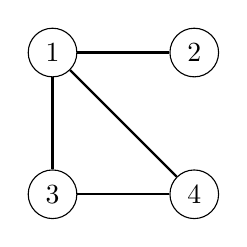
\begin{tikzpicture}[scale=0.9]
\node[draw, circle] (1) at (1,3) {$1$};
\node[draw, circle] (2) at (3,3) {$2$};
\node[draw, circle] (3) at (1,1) {$3$};
\node[draw, circle] (4) at (3,1) {$4$};

\path[draw,thick,-] (1) -- (2);
\path[draw,thick,-] (1) -- (3);
\path[draw,thick,-] (3) -- (4);
\path[draw,thick,-] (1) -- (4);
\end{tikzpicture}
\end{center}
Tällä verkolla on kolme virittävää puuta:
\begin{center}
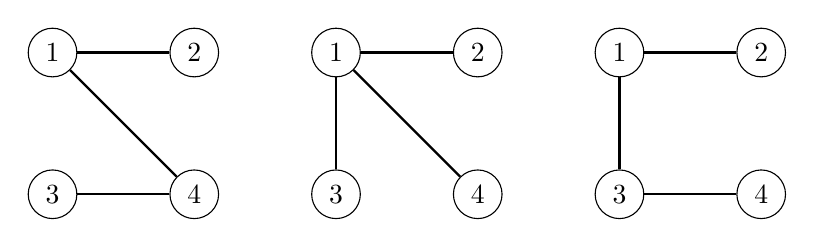
\begin{tikzpicture}[scale=0.9]
\node[draw, circle] (1a) at (1,3) {$1$};
\node[draw, circle] (2a) at (3,3) {$2$};
\node[draw, circle] (3a) at (1,1) {$3$};
\node[draw, circle] (4a) at (3,1) {$4$};

\path[draw,thick,-] (1a) -- (2a);
%\path[draw,thick,-] (1a) -- (3a);
\path[draw,thick,-] (3a) -- (4a);
\path[draw,thick,-] (1a) -- (4a);

\node[draw, circle] (1b) at (1+4,3) {$1$};
\node[draw, circle] (2b) at (3+4,3) {$2$};
\node[draw, circle] (3b) at (1+4,1) {$3$};
\node[draw, circle] (4b) at (3+4,1) {$4$};

\path[draw,thick,-] (1b) -- (2b);
\path[draw,thick,-] (1b) -- (3b);
%\path[draw,thick,-] (3b) -- (4b);
\path[draw,thick,-] (1b) -- (4b);

\node[draw, circle] (1c) at (1+8,3) {$1$};
\node[draw, circle] (2c) at (3+8,3) {$2$};
\node[draw, circle] (3c) at (1+8,1) {$3$};
\node[draw, circle] (4c) at (3+8,1) {$4$};

\path[draw,thick,-] (1c) -- (2c);
\path[draw,thick,-] (1c) -- (3c);
\path[draw,thick,-] (3c) -- (4c);
%\path[draw,thick,-] (1c) -- (4c);
\end{tikzpicture}
\end{center}

Muodostetaan verkosta Laplacen matriisi $L$,
jossa $L[i,i]$ on solmun $i$ aste ja
$L[i,j]=-1$, jos solmujen $i$ ja $j$ välillä on kaari,
ja muuten $L[i,j]=0$.
Tässä tapauksessa matriisista tulee

\[
L= \begin{bmatrix}
  3 & -1 & -1 & -1 \\
  -1 & 1 & 0 & 0 \\
  -1 & 0 & 2 & -1 \\
  -1 & 0 & -1 & 2 \\
 \end{bmatrix}.
\]

Nyt virittävien puiden määrä on determinantti
matriisista, joka saadaan poistamasta matriisista $L$
jokin rivi ja jokin sarake.
Esimerkiksi jos poistamme ylimmän rivin ja
vasemman sarakkeen, tuloksena on

\[ \det(
\begin{bmatrix}
  1 & 0 & 0 \\
  0 & 2 & -1 \\
  0 & -1 & 2 \\
 \end{bmatrix}
) =3.\]

Determinantista tulee aina sama riippumatta siitä,
mikä rivi ja sarake matriisista $L$ poistetaan.

Huomaa, että Kirchhoffin lauseen erikoistapauksena on
luvun 22.6 Cayleyn kaava, koska voidaan osoittaa, että
täydellisessä $n$ solmun verkossa

\[ \det(
\begin{bmatrix}
  n-1 & -1 & \cdots & -1 \\
  -1 & n-1 & \cdots & -1 \\
  \vdots & \vdots & \ddots & \vdots \\
  -1 & -1 & \cdots & n-1 \\
 \end{bmatrix}
) =n^{n-2}.\]

